\chapter{Introduction}
\section{Problem statement and motivation}
The following gives some superficial instructions for using this template for a Master's thesis. For guidelines on thesis writing you can consult various sources, for example, the Bachelor thesis template.

The thesis should have an introduction chapter. Other chapters can be named according to the topic. In the end, some summary chapter is needed; see Chapter~\ref{chapter:conclusions} for an example.

\section{Structure of thesis}
Cool stuff etc.

\chapter{Neural networks}
Background stuff 
\section{Fully Connected Networks}
When needed example of a transfer learning head?, when good/bad
\section{Convolutional Neural Networks}
Show some basic CNN things maybe and why needed over fully connected bois :) 
\subsection{Neural image processing}
How it different from classical features and how/why it works
\section{Attention}
Attention huh
\section{Multi-task learning}
Describe how a multi-task setting differs or maybe in the other chapter only?
\section{RNN/LSTM/Transformer text processing/generation}
Depending on what may be used

\chapter{Image classification}
Image classification is one of the essential modern computer vision problems, where the goal is to create a model that can classify an input image into one of a set of pre-defined classes. Before the popularization of applying large Convolutional Neural Networks for this task, the most successful way of solving the problem was to use some algorithm for finding feature descriptors in a set of images to construct a Visual Bag of Words.  A linear classifier, like a Support Vector Machine, would then do the classification using the Bag of Words representation of an image. These days nearly all approaches are based on using deep CNNs, and working CNNs were deployed already in 1998 on character recognition in the form of LeNet \citep{leNet}.
\section{ImageNet}
ImageNet  \citep{imagenet}  is perhaps the most significant dataset for image classification and especially the ImageNet Challenge \citep{ILSVRC}, which is a challenge for a collection of 1000 classes from the ImageNet dataset for image classification using 1.2 million training and 150 thousand  images of the entire ImageNet dataset. In 2012 the winning model, AlexNet \citep{alexNet}, showed that it was possible to train a deep CNNs efficiently using GPUs. Since 2012 all top-performing models showed some new improvements on how to create the most performant network architecture, for example, VGGNet from the year 2014 and ResNet \citep{resNet} from 2015, both of which have been popular models to use for Transfer Learning since.

Human accuracy on the ImageNet challenge is about 5.1\% \citep{imageNet_summary}, and ResNet achieves a top-5 error rate of 3.57\% \citep{resNet} and newer architectures even lower, but this still does not mean that image classification is a solved problem. The human performance experiment found that many of the human errors are caused by not having expert information in, for example, identifying animal species or not even being aware of the existence of a class \citep{imageNet_summary}. ObjectNet \citep{objectNet} is a dataset designed to  image classifiers with a focus on their generalizability. It contains many classes that also exist in the ImageNet dataset. However, they are in unexpected locations or have an unexpected pose, causing the high accuracy image classifiers trained on ImageNet experience a 40-45\% accuracy drop when evaluating them on the ObjectNet images of classes shared between ImageNet and ObjectNet. This kind of adjustment is relatively easy for a human, and it shows that while the classifiers are good, they are by no means perfect.
\section{Transfer learning}
Unlike the ImageNet challenge, most real-world tasks do not have such an abundance of data for all possible classes. Still, to achieve the highest accuracies, they require models that are equal in terms of complexity to those that have top accuracies problems on the scale of the ImageNet classification. For this reason, many CNN classifiers, irrespective of the problem, feature one of the ImageNet classifiers in the model architecture. Even though some datasets may contain a large number of images per class, using a pre-trained classifier as a basis often produces a better final classifier by applying fine-tuning \citep{betterTransfer}.

The idea behind transfer learning is to train on a related task to the end task first. Then the network weights in the model for the actual task are initialized to those of the model we are transferring from, so the training of the original model is a pre-step to the real task. Since training the models on ImageNet scale datasets is not generally feasible due to their large number of parameters and long training time, one of the pre-trained models is picked and then fine-tuned. Fine-tuning a classifier means taking the examples for the final task, and training the network on those, updating the original classifier at the same time. The transfer learning approach differs significantly from the traditional learning model, where each task requires a separate model that learns from the given data using random weights. Since image inputs are often very high dimensional, the traditional approach may not work in many cases. The pre-training allows for focusing on data that provides answers to the actual task and not on learning low-level features, which the ImageNet classifiers would already have learned.

\begin{figure}[h!] 
\centering 
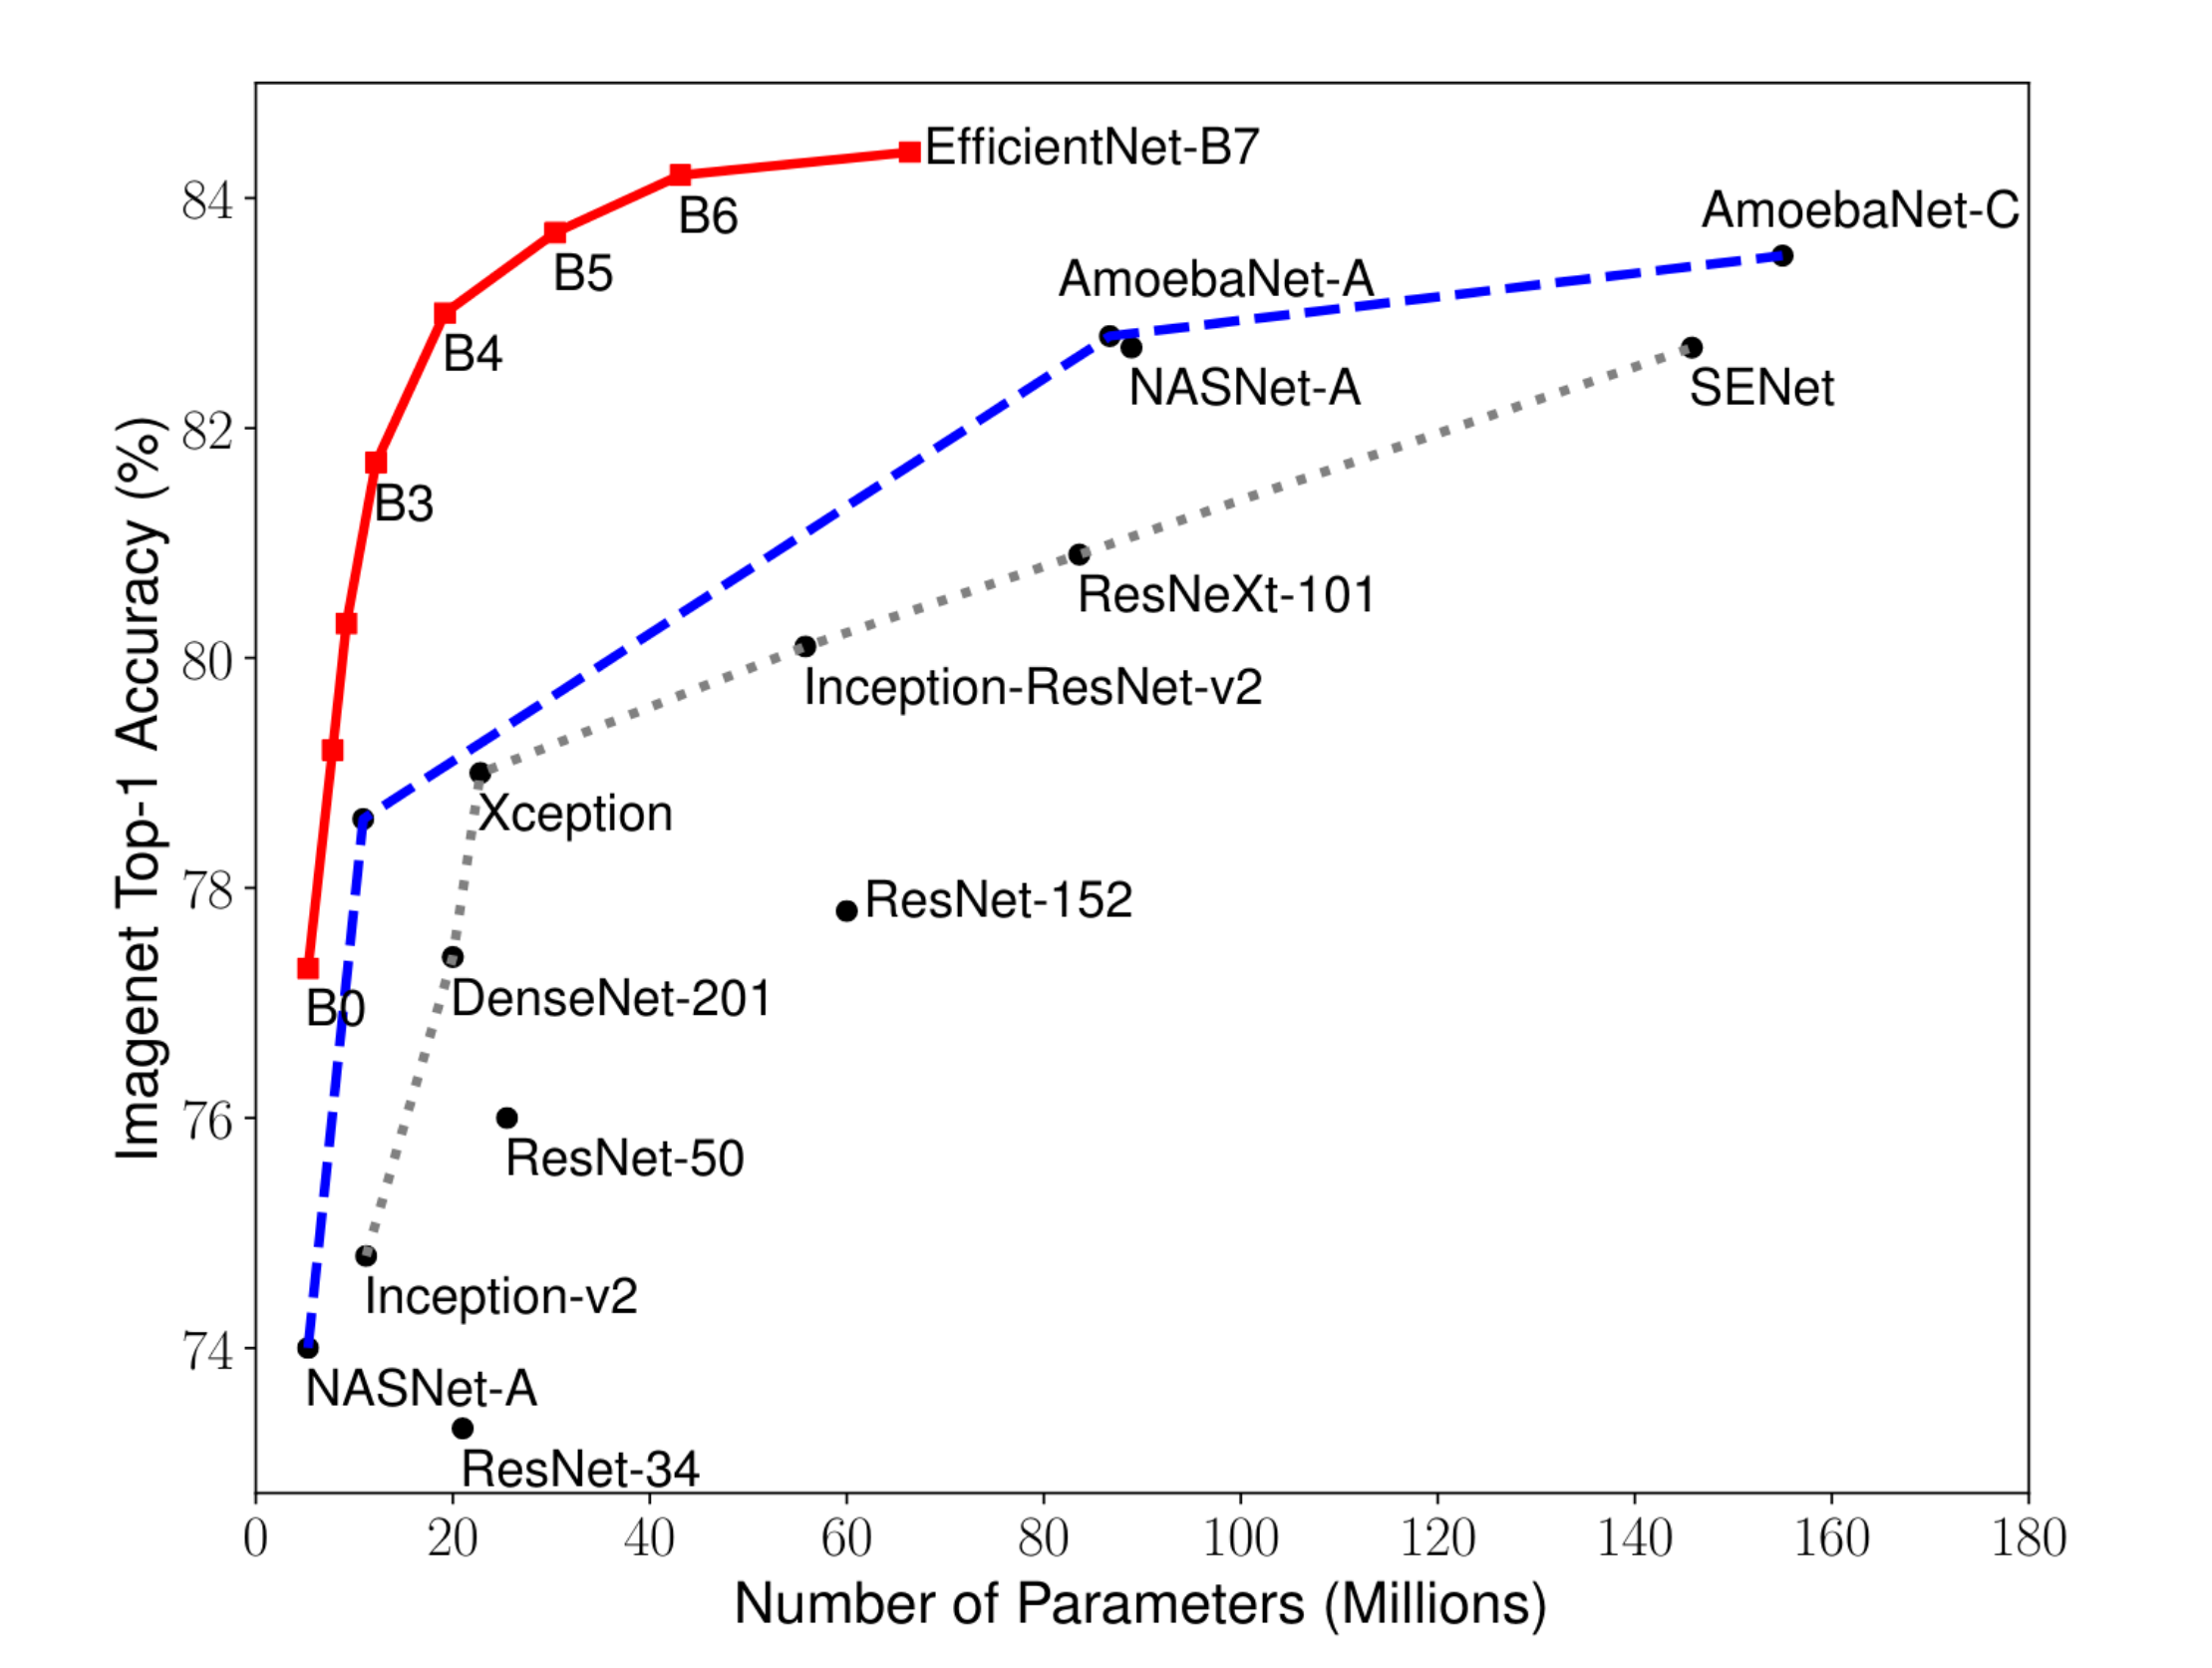
\includegraphics[width=0.8\textwidth]{imgs/imagenet_parameters.png}
\caption{Number of parameters in popular ImageNet classifiers. Figure from \citep{efficientNet}.\label{fig:params}}
\end{figure}

Picking which classifier to use as a base is often problem-dependent. As it is not possible to declare one network structure to be the best at all tasks, picking the best model to start with usually requires the user to compare different architectures and weighing the requirements for the problem at hand. Often though, the larger models will perform better, and there exists a correlation between performing well on ImageNet and being a good transfer learning model \citep{betterTransfer}. Though as can be seen in figure 3.1, better performance often comes at the cost of many more parameters, requiring more memory to train the model. Though just the number of parameters is not the only thing to compare as the throughput of a Resnet50 turns out to be about three times as large as the throughput of an EfficientNet-B4 even though they have a similar amount of parameters \citep{classifierPerformance}.

If there is enough data, it turns out that using a pre-trained network does not provide any benefits in terms of the converged model accuracy, but it is not detrimental to performance either \citep{rethinkTransfer}. When training sufficiently long on a sufficient amount of data, the pre-trained and randomly initialized networks converged to similar accuracies but required significantly different amounts of training resources. Still, this does not mean that pre-training is useless by any means as the saved resources and getting models to converge faster are essential factors for progress, and of course, in many cases, training from scratch will not provide satisfying results.

To formally define transfer learning, let $\mathcal{D}$ be a domain for the features, in this case, images.
\section{ResNet}
\section{EfficientNet}
\chapter{Object detection}
Based on what is going to be detected, maybe text, cars, people?
\chapter{Paragraph captioning}
Assuming we are doing this
\chapter{Multi task learning}
Cover some examples of MTL in Computer Vision, differences to Transfer Learning, why it might work, why we might see detrimental results

\chapter{Datasets}
Describing our data
\section{Data formats}
Describe what datasets are used for each of the tasks and where they are from etc.

\chapter{Experiments}
Here are our experiments
\section{Training process}
\subsection{Evaluation criterias}
eval
\section{Image classifiers}
Results of image classsifiers on the datasets maybe compare ResNet vs EfficientNet
\subsection{Only transfer learned classifier}
Just a ResNet or something
\subsection{Image classifier with attention}
Add attention to image classifier
\subsection{Classifiers combined to a multi-task model}
How it do
\section{Object detection}
Some stuff for object detection
\section{Multi-task models}
Create multi-task models for all and try to find some pairs/tuples that actually work together properly
\chapter{Result analysis}
Incredible models absolutely.

\chapter{Future work}
How to make it better what could be tried 

\chapter{Figures and Tables}

\section{Figures}
Figure~\ref{fig:logo} gives an example how to add figures to the document. Remember always to cite the figure in the main text.

\begin{figure}[h!] 
\centering 
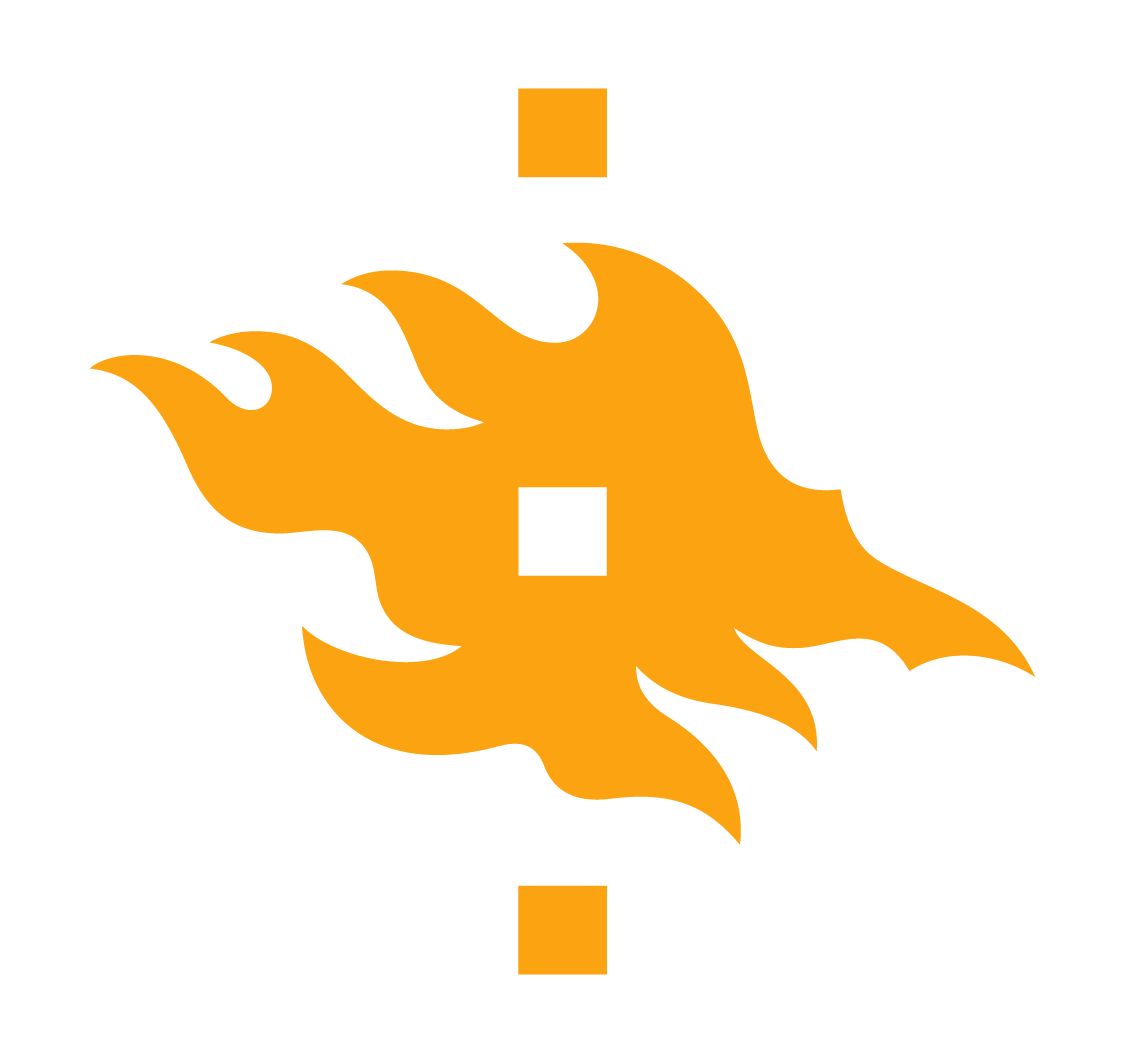
\includegraphics[width=0.3\textwidth]{HY-logo-ml.png}
\caption{University of Helsinki flame-logo for Faculty of Science.\label{fig:logo}}
\end{figure}

\section{Tables}

Table~\ref{table:results} gives an example how to report experimental results. Remember always to cite the table in the main text. 

\begin{table}
\centering
\caption{Experimental results.\label{table:results}}
\begin{tabular}{l||l c r} 
Experiment & 1 & 2 & 3 \\ 
\hline \hline 
$A$ & 2.5 & 4.7 & -11 \\
$B$ & 8.0 & -3.7 & 12.6 \\
$A+B$ & 10.5 & 1.0 & 1.6 \\
\hline
%
\end{tabular}
\end{table}

\chapter{Citations}

\section{Citations to literature}

References are listed in a separate .bib-file. In this case it is named \texttt{bibliography.bib} including the following content:
\begin{verbatim}
@article{einstein,
    author =       "Albert Einstein",
    title =        "{Zur Elektrodynamik bewegter K{\"o}rper}. ({German})
        [{On} the electrodynamics of moving bodies]",
    journal =      "Annalen der Physik",
    volume =       "322",
    number =       "10",
    pages =        "891--921",
    year =         "1905",
    DOI =          "http://dx.doi.org/10.1002/andp.19053221004"
}
 
@book{latexcompanion,
    author    = "Michel Goossens and Frank Mittelbach and Alexander Samarin",
    title     = "The \LaTeX\ Companion",
    year      = "1993",
    publisher = "Addison-Wesley",
    address   = "Reading, Massachusetts"
}
 
@misc{knuthwebsite,
    author    = "Donald Knuth",
    title     = "Knuth: Computers and Typesetting",
    url       = "http://www-cs-faculty.stanford.edu/%7Eknuth/abcde.html"
}
1
\end{verbatim}

In the last reference url field the code \verb+%7E+ will translate into \verb+~+ once clicked in the final pdf.

References are created using command \texttt{\textbackslash cite\{einstein\}}, showing as \citep{einstein}. Other examples: \citep{latexcompanion,knuthwebsite}.

Citation style can be negotiated with the supervisor. See some options in \url{https://www.sharelatex.com/learn/Bibtex_bibliography_styles}.

\section{Crossreferences}

Appendix~\ref{appendix:model} on page~\pageref{appendix:model} contains some additional material.

\chapter{From tex to pdf}

In Linux, run \texttt{pdflatex filename.tex} and \texttt{bibtex filename.tex} repeatedly until no more warnings are shown. This process can be automised using make-command.
 
\chapter{Conclusions\label{chapter:conclusions}}

It is good to conclude with a summary of findings. You can also use separate chapter for discussion and future work. These details you can negotiate with your supervisor.